\documentclass[10pt,twocolumn,letterpaper]{article}

\usepackage{cvpr}
\usepackage{times}
\usepackage{epsfig}
\usepackage{graphicx}
\usepackage{amsmath}
\usepackage{amssymb}

\usepackage{url}

% Include other packages here, before hyperref.
\usepackage{algorithm}
\usepackage{algpseudocode}
% If you comment hyperref and then uncomment it, you should delete
% egpaper.aux before re-running latex.  (Or just hit 'q' on the first latex
% run, let it finish, and you should be clear).
%\usepackage[pagebackref=true,breaklinks=true,letterpaper=true,colorlinks,bookmarks=false]{hyperref}

\cvprfinalcopy % *** Uncomment this line for the final submission

\def\cvprPaperID{****} % *** Enter the CVPR Paper ID here
\def\httilde{\mbox{\tt\raisebox{-.5ex}{\symbol{126}}}}

% Pages are numbered in submission mode, and unnumbered in camera-ready
\ifcvprfinal\pagestyle{empty}\fi
\begin{document}

\title{Comparison between a sequential and a multithreading version of the mean shift clustering algorithm}

\author{Emilio Cecchini\\
{\tt\small emilio.cecchini@stud.unifi.it}
}


\maketitle
\thispagestyle{empty}


\begin{abstract}
In this paper, after a brief introduction to the mean shift clustering, a sequential version will be compared with a multithreading version of the algorithm. The obtained speedup with a multi-core CPU will be analyzed using a different number of threads. The algorithm is written in C++ and the parallel version is obtained with OpenMP. The focus of this paper and his associated code do not consist in showing a very efficient version of the mean shift clustering algorithm, but rather in analyzing the performance improvements obtainable with a  multithreading version compared to a sequential one.
\end{abstract}

\section{Introduction}

Since there are many variations of the mean shift algorithm, in this section I will describe the specific version used in my implementation.

%-------------------------------------------------------------------------
\subsection{Mean shift}

The mean shift algorithm is a nonparametric clustering technique that does not require as input the number of clusters to look for.  It is based on the concept of \textit{kernel density estimation} or \textit{KDE}, that is a method to estimate the underlying distribution for a set of data.

At each step, a \textit{kernel function} is applied to each point that causes the points to shift in the direction of the local maxima determined by the kernel. The iterations end when all points reach the maxima of the underlying distribution estimated by the chosen kernel.

There are many different types of kernel, the most used is the \textit{Gaussian kernel}:

\begin{align}
k(x) =  e^{-\dfrac{x}{2\sigma^2}}
\end{align}

The standard deviation $\sigma$ is the \textit{bandwidth} parameter. Depending on the kernel bandwidth parameter used, the resultant density function will vary: with a high bandwith value you will get a few large clusters and vice versa.

The new location where to shift each point at each step of the algorithm is computed as a weighted average between the point and its neighbors, where the weights are calculated with the Gaussian kernel. Suppose $x$ is a point to be shifted and $N(x)$ are the sets of points near to that point. Let $dist(x, x_i)$ be the distance from the point $x$ to the point $x_i$. The new position $x'$ where $x$ has to be shifted is computed as follows:

\begin{align}
x' = \dfrac{\sum_{x_i \in N(x)} k(dist(x,x_i)^2) x_i}{\sum_{x_i \in N(x)} k(dist(x, x_i)^2)}
\end{align}

The mean shift algorithm applies that formula to each point iteratively until they converge, that is until the position does not change.

\subsection{The algorithm}

The algorithm is very simple: each point shifts towards the maxima of its underlying distribution. The algorithm ends when all the points have stopped shifting.

Here is the pseudocode of the core of the algorithm:

\begin{algorithm}
\label{MeanShiftAlgSeq}
\caption{Mean shift core}
\begin{algorithmic}

	\While{allPointsHaveStoppedShifting()}
    		\For{each point $p$}
    			\If{hasStoppedShifting($p$)}
    				\State \textbf{continue}
    			\EndIf
    		\State shift($p$)
    		\EndFor
    \EndWhile

\end{algorithmic}
\end{algorithm}

To speed up the process, the shifting process of a point is stopped when the distance from its older position is less than an epsilon value specified by the user.


\subsection{The parallel version}

The mean shift algorithm is a embarrassingly parallel work: each point perform its shifting independently from the other points. This makes it the perfect case for using the OpenMP technology. In fact, with a single \verb"pragma" command it was possible to switch from a sequential version to a parallel version.

Here is the pseudocode of the parallel version of the core algorithm:

\begin{algorithm}
\label{MeanShiftAlgPar}
\caption{Mean shift core parallel}
\begin{algorithmic}

	\While{allPointsHaveStoppedShifting()}
		\State \#pragma omp parallel for schedule(dynamic)
    		\For{each point $p$}
    			\If{hasStoppedShifting($p$)}
    				\State \textbf{continue}
    			\EndIf
    		\State shift($p$)
    		\EndFor
    \EndWhile

\end{algorithmic}
\end{algorithm}

Note that the only difference from the sequential version in \ref{MeanShiftAlgSeq} is the \verb"pragma" statement. That statement is placed just before the \verb"for" loop, in this way there is no need of any critical sections. If it had been placed before the \verb"while" loop, then the parallel algorithm would have been more complex introducing an overhead due to the synchronization between threads.

The clause \verb"schedule(dynamic)" is important because at the end of the computation, there will be some points that have stopped shifting, so they immediatly end the computation of the for loop. With the dynamic scheduling there will be a better distribution of the workload of each thread.

\subsection{Speedup analysis}

The speedup is computed with a script that first executes a sequential version, then it executes on the same data set differents parallel versions using a different number of threads. 

Here is a table and a chart reporting the speedup of the parallel version with a different number of threads. The test was performed on a machine with an Intel Xeon CPU 2.00 \textit{GHz} with 8 cores on a data set of $10000$ points of three dimensions:
\\
\\
\textbf{Sequential version}: 54.1719 \textit{s}
\\

\begin{table}[H]
\centering
\begin{tabular}{ccc}
\hline
 \textbf{Threads} & \textbf{Time} (seconds) & \textbf{Speedup} \\
\hline
2 & 27.42 & 1.98 \\
3 & 18.36 & 2.95 \\
4 & 13.72 & 3.95 \\
5 & 12.44 & 4.35 \\
6 & 12.25 & 4.42 \\
7 & 10.83 & 5.00 \\
8 & 10.11 & 5.36 \\
9 & 10.50 & 5.16 \\
10 & 10.42 & 5.20 \\
\hline
\end{tabular}
\end{table}

\begin{figure}[H]
\centering
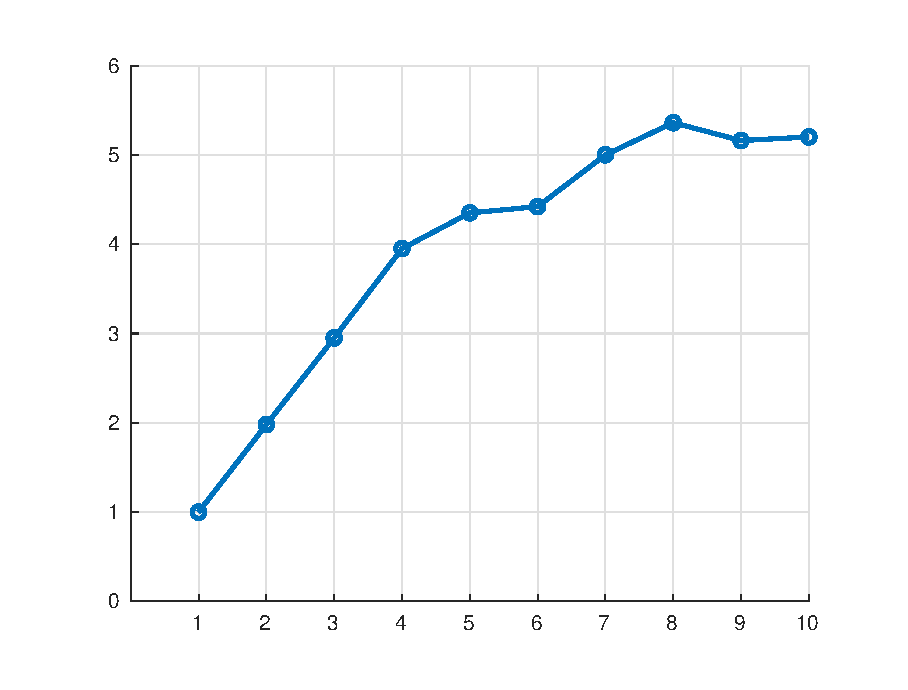
\includegraphics[width=3.2in]{speedup.eps}
\end{figure}

The speedup seems to grow with three different patterns. From two threads to four threads the speeup is almost perfectly linear, from five to eight it seems to be sub-linear and over eight threads it stops growing.

\begin{figure}[H]
\centering
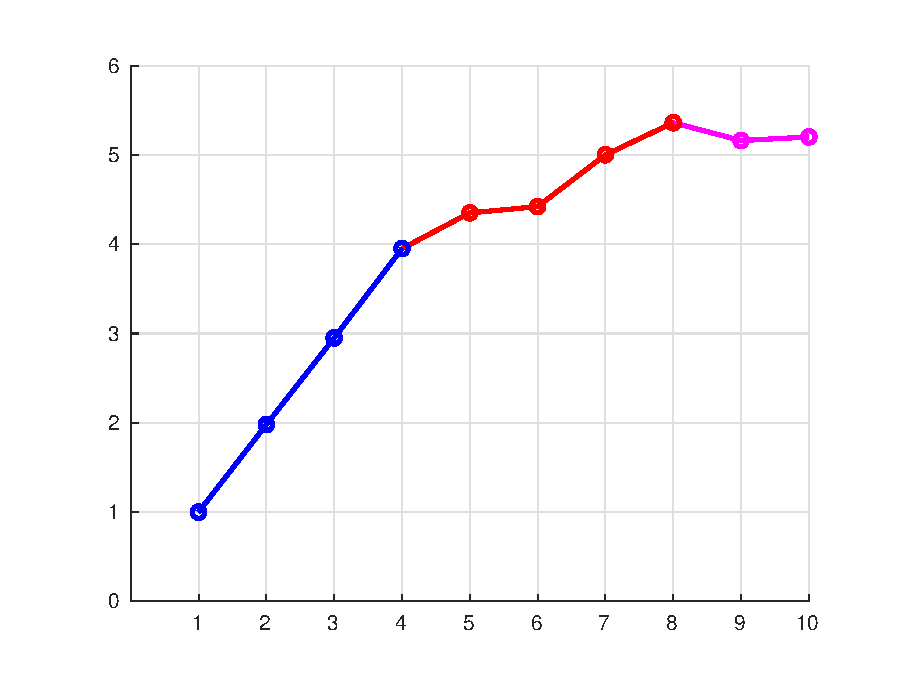
\includegraphics[width=3.2in]{speedup_colors.eps}
\end{figure}

The explanation for these three different growing trends is immediate. The machine where the test was performed has the hyperthreading technology enabled: it shows eight cores but actually it has only four physical cores, the other four cores are virtual. In fact, from two to four threads the speedup is linear because each physical core has to execute a single thread. Using from five to eight threads can speed up the execution, but the speedup is no more perfectly linear, because there are more threads than physical cores. Finally over eight threads there is no more improvements in terms of speeds, on the contrary, it is slightly slower due to the overhead of the contex switches between threads.
\end{document}
